\documentclass[11pt]{article}
\usepackage[latin2]{inputenc}
\usepackage{a4wide}
\usepackage{graphicx}
\usepackage{hyperref}
\hypersetup{colorlinks=true,linkcolor=blue}
\title{Low Profile Thumb Prosthesis Documentation}
\author{ThingDoc}

\begin{document}

\maketitle
\begin{center}

\includegraphics[width=8cm]{logo.png}
\end{center}
This prosthesis is designed to provide a static thumb post for patients who have one or more fingers with a good range of motion, but no thumb to oppose against. The prosthesis consists of a silicone sleeve that goes around the patient's palm, tightened by a velcro strap. A mounting point for a static thumb post (optionally with a grippy silicone cover) is molded into the sleeve.

\newpage

\tableofcontents

\newpage

\section{Bill of Materials}
List of things you need to build the machine divided by categories.

\subsection{Prerequisites!}
\begin{itemize}
\item 1x \hyperlink{thing_hand\_scan}{3D scan of patient's hand}
\end{itemize}

\subsection{Materials}
\begin{itemize}
\item 100x \hyperlink{thing_g\_dragon\_skin\_30}{grams of Dragon Skin 30 liquid silicone}
\item 10x \hyperlink{thing_g\_dragon\_skin\_10}{grams of Dragon Skin 10 liquid silicone}
\end{itemize}

\subsection{Fasteners}
\begin{itemize}
\item 4x M4 Hex Nut
\item 1x \hyperlink{thing_velcro\_strap}{Velcro Strap}
\item 6x Piece of Tape
\item 4x M4x15 Bolt
\end{itemize}

\subsection{Printed}
\begin{itemize}
\item 2x \hyperlink{thing_rigid\_base}{Rigid base with thumb}
\item 1x \hyperlink{thing_mold\_left\_half}{Mold - left half}
\item 1x \hyperlink{thing_truncated\_hand}{Truncated Print of Patient's Hand}
\item 1x \hyperlink{thing_thumb\_mold}{Thumb Mold}
\item 1x \hyperlink{thing_mold\_right\_half}{Mold - right half}
\end{itemize}

\newpage

\section{Things Overview}
List of things and their descriptions.

\hypertarget{thing_config\_file}{\subsection{Configuration and Rendering of 3D models}}
Configuration settings for the Shriners Hand, required to generate correct STLs of the printed parts. See the Configuration File Assembly instructions to set this up.

\hypertarget{thing_rigid\_base}{\subsection{Rigid base with thumb}}
3D printed rigid base and static thumb post - rendered from src/scad/rigid_base.scad
\includegraphics[width=4cm]{images/rigid\_base.png}

\hypertarget{thing_silicone\_sleeve}{\subsection{Silicone sleeve}}
Silicone sleeve that goes over the patient's palm

\hypertarget{thing_molded\_thumb}{\subsection{Thumb with Molded Grip}}
Molded silicone thumb pad can improve grip and provide some tactile feedback to the wearer

\hypertarget{thing_truncated\_hand}{\subsection{Truncated Print of Patient's Hand}}
Shortened and resized portion of the patient's palm to be the center of the mold during silicone casting - rendered from src/scad/truncated_hand.scad (example shown)
\includegraphics[width=4cm]{images/truncated\_hand.png}

\hypertarget{thing_thumb\_mold}{\subsection{Thumb Mold}}
Mold for casting the silicone finger tip grip - rendered from src/inventor/thumb_mold.ipt
\includegraphics[width=4cm]{images/thumb\_mold.png}

\hypertarget{thing_g\_dragon\_skin\_10}{\subsection{grams of Dragon Skin 10 liquid silicone}}
Dragon Skin 10 silicone resin kit, available from Smooth-On. Shore A durometer (hardness) 10.
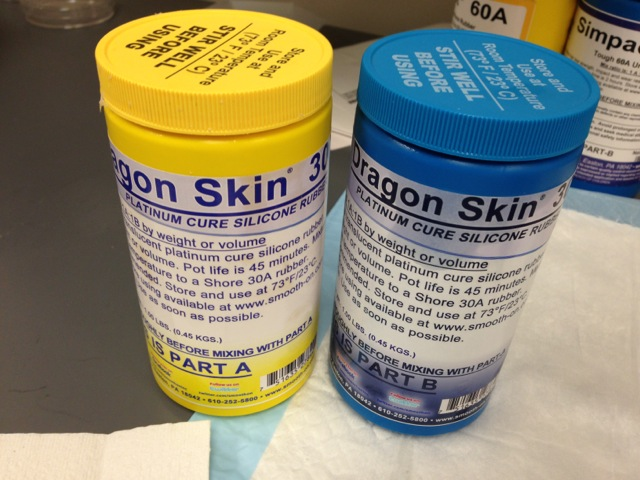
\includegraphics[width=4cm]{images/pad\_casting/DragonSkin.jpg}

\hypertarget{thing_mold\_right\_half}{\subsection{Mold - right half}}
Right half of 3D printed mold for casting the silicone sleeve - rendered from src/scad/mold_right.scad
\includegraphics[width=4cm]{images/mold\_right\_half.png}

\hypertarget{thing_mold\_left\_half}{\subsection{Mold - left half}}
Left half of 3D printed mold for casting the silicone sleeve - rendered from src/scad/mold_left_half.scad
\includegraphics[width=4cm]{images/mold\_left\_half.png}

\hypertarget{thing_g\_dragon\_skin\_30}{\subsection{grams of Dragon Skin 30 liquid silicone}}
Dragon Skin 30 silicone resin kit, available from Smooth-On. Shore A durometer (hardness) 30.
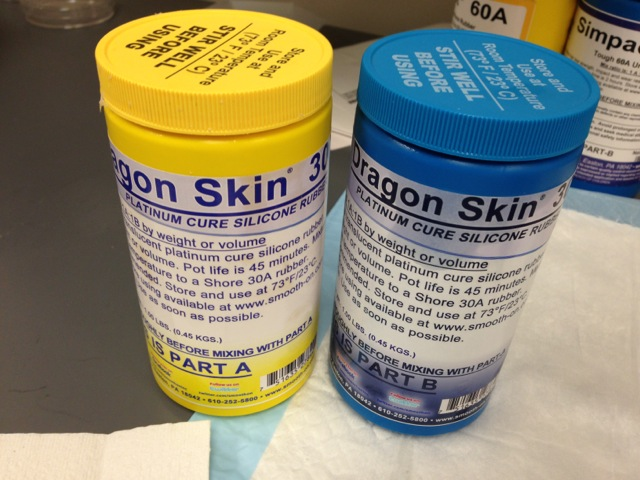
\includegraphics[width=4cm]{images/pad\_casting/DragonSkin.jpg}

\hypertarget{thing_velcro\_strap}{\subsection{Velcro Strap}}
9mm wide velcro strap of adequate length to wrap around the patient's palm with at least 30% extra.

\hypertarget{thing_hand\_scan}{\subsection{3D scan of patient's hand}}
3D scan of the patient's hand with wrist and finger(s) held straight. Must be a manifold mesh (STL file); may be simplified for faster processing. Place in userScans directory before configuring and rendering OpenSCAD models.

\hypertarget{thing_mold\_assembly}{\subsection{Palm Sleeve Mold Assembly}}
Assembled mold for casting the silicone sleeve

\newpage

\section{Assembly Instructions}

\subsection{Assemble Configuration and Rendering of 3D models}
Things needed:
\begin{itemize}
\item 1x \hyperlink{thing_hand\_scan}{3D scan of patient's hand}
\end{itemize}
Steps:
\begin{enumerate}
\item Place a manifold, cleaned-up version of the patient's hand scan in the userScans folder.
\item Open src/scad/configuration.scad in your favorite text editor.
\item Type the filename of the patient's hand scan in place of "JudahLeftHandShortened.stl" in the configuration file.
\item Open alignment.scad using OpenSCAD so you can see the placement of the 3D model while you edit the configuration file. (you may have to manually press the Reload and Preview button every time you make a change to the configuration file)
\item Change the hand\_d parameter to the diameter of the thickest part of the patient's hand in mm.
\item Adjust the hand\_pos (position of the hand in 3D space) and hand\_rot (rotation of hand around each axis) parameters so that the 3D scan of the hand is aligned with the arrows as described in the following steps.
\item The palm of the hand should be roughly vertical, centered on the green crosshair as much as possible, and the hand should be oriented so that the patient's finger(s) flex toward the green arrow.\\ 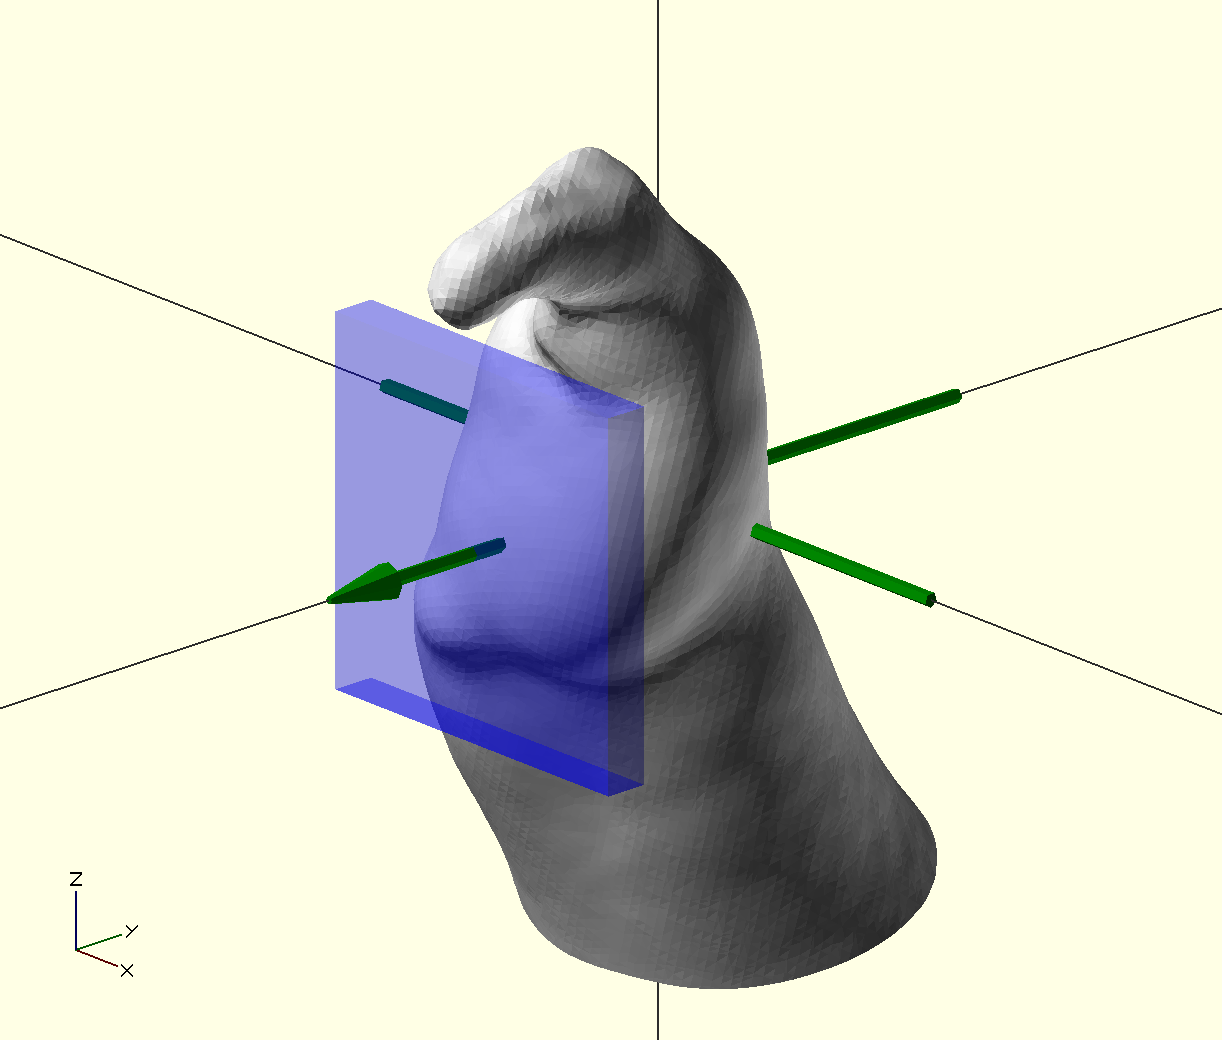
\includegraphics[width=4cm]{images/configuration/positioning.png}
\item The palmar surface should be just within the blue area when viewed from the side.\\ \includegraphics[width=4cm]{images/configuration/forward\_alignment.png}
\item (Optional) Adjust the other parameters in the configuration file to control the dimensions of various parts of the prosthesis. The default values should work most of the time.
\item After you have aligned the hand, open src/scad/preview.scad in OpenSCAD to ensure that all parts of the prosthesis look correct.\\ \includegraphics[width=4cm]{images/configuration/assembly\_preview.png}
\item Open each part to be printed (from the src/scad folder) in OpenSCAD, render each one (F6) and export as STL, then print using the STL files.
\end{enumerate}

\subsection{Assemble Palm Sleeve Mold Assembly}
Things needed:
\begin{itemize}
\item 1x \hyperlink{thing_config\_file}{Configuration and Rendering of 3D models}
\item 4x M4 Hex Nut
\item 1x \hyperlink{thing_mold\_left\_half}{Mold - left half}
\item 1x \hyperlink{thing_rigid\_base}{Rigid base with thumb}
\item 4x Piece of Tape
\item 1x \hyperlink{thing_mold\_right\_half}{Mold - right half}
\item 4x M4x15 Bolt
\end{itemize}
Steps:
\begin{enumerate}
\item Set one half of the mold on a flat surface with the flat side down.
\item Insert the rigid thumb base into the slot in the side of the mold, with the round part toward the inside and the shorter prong toward the closed end of the mold.\\ 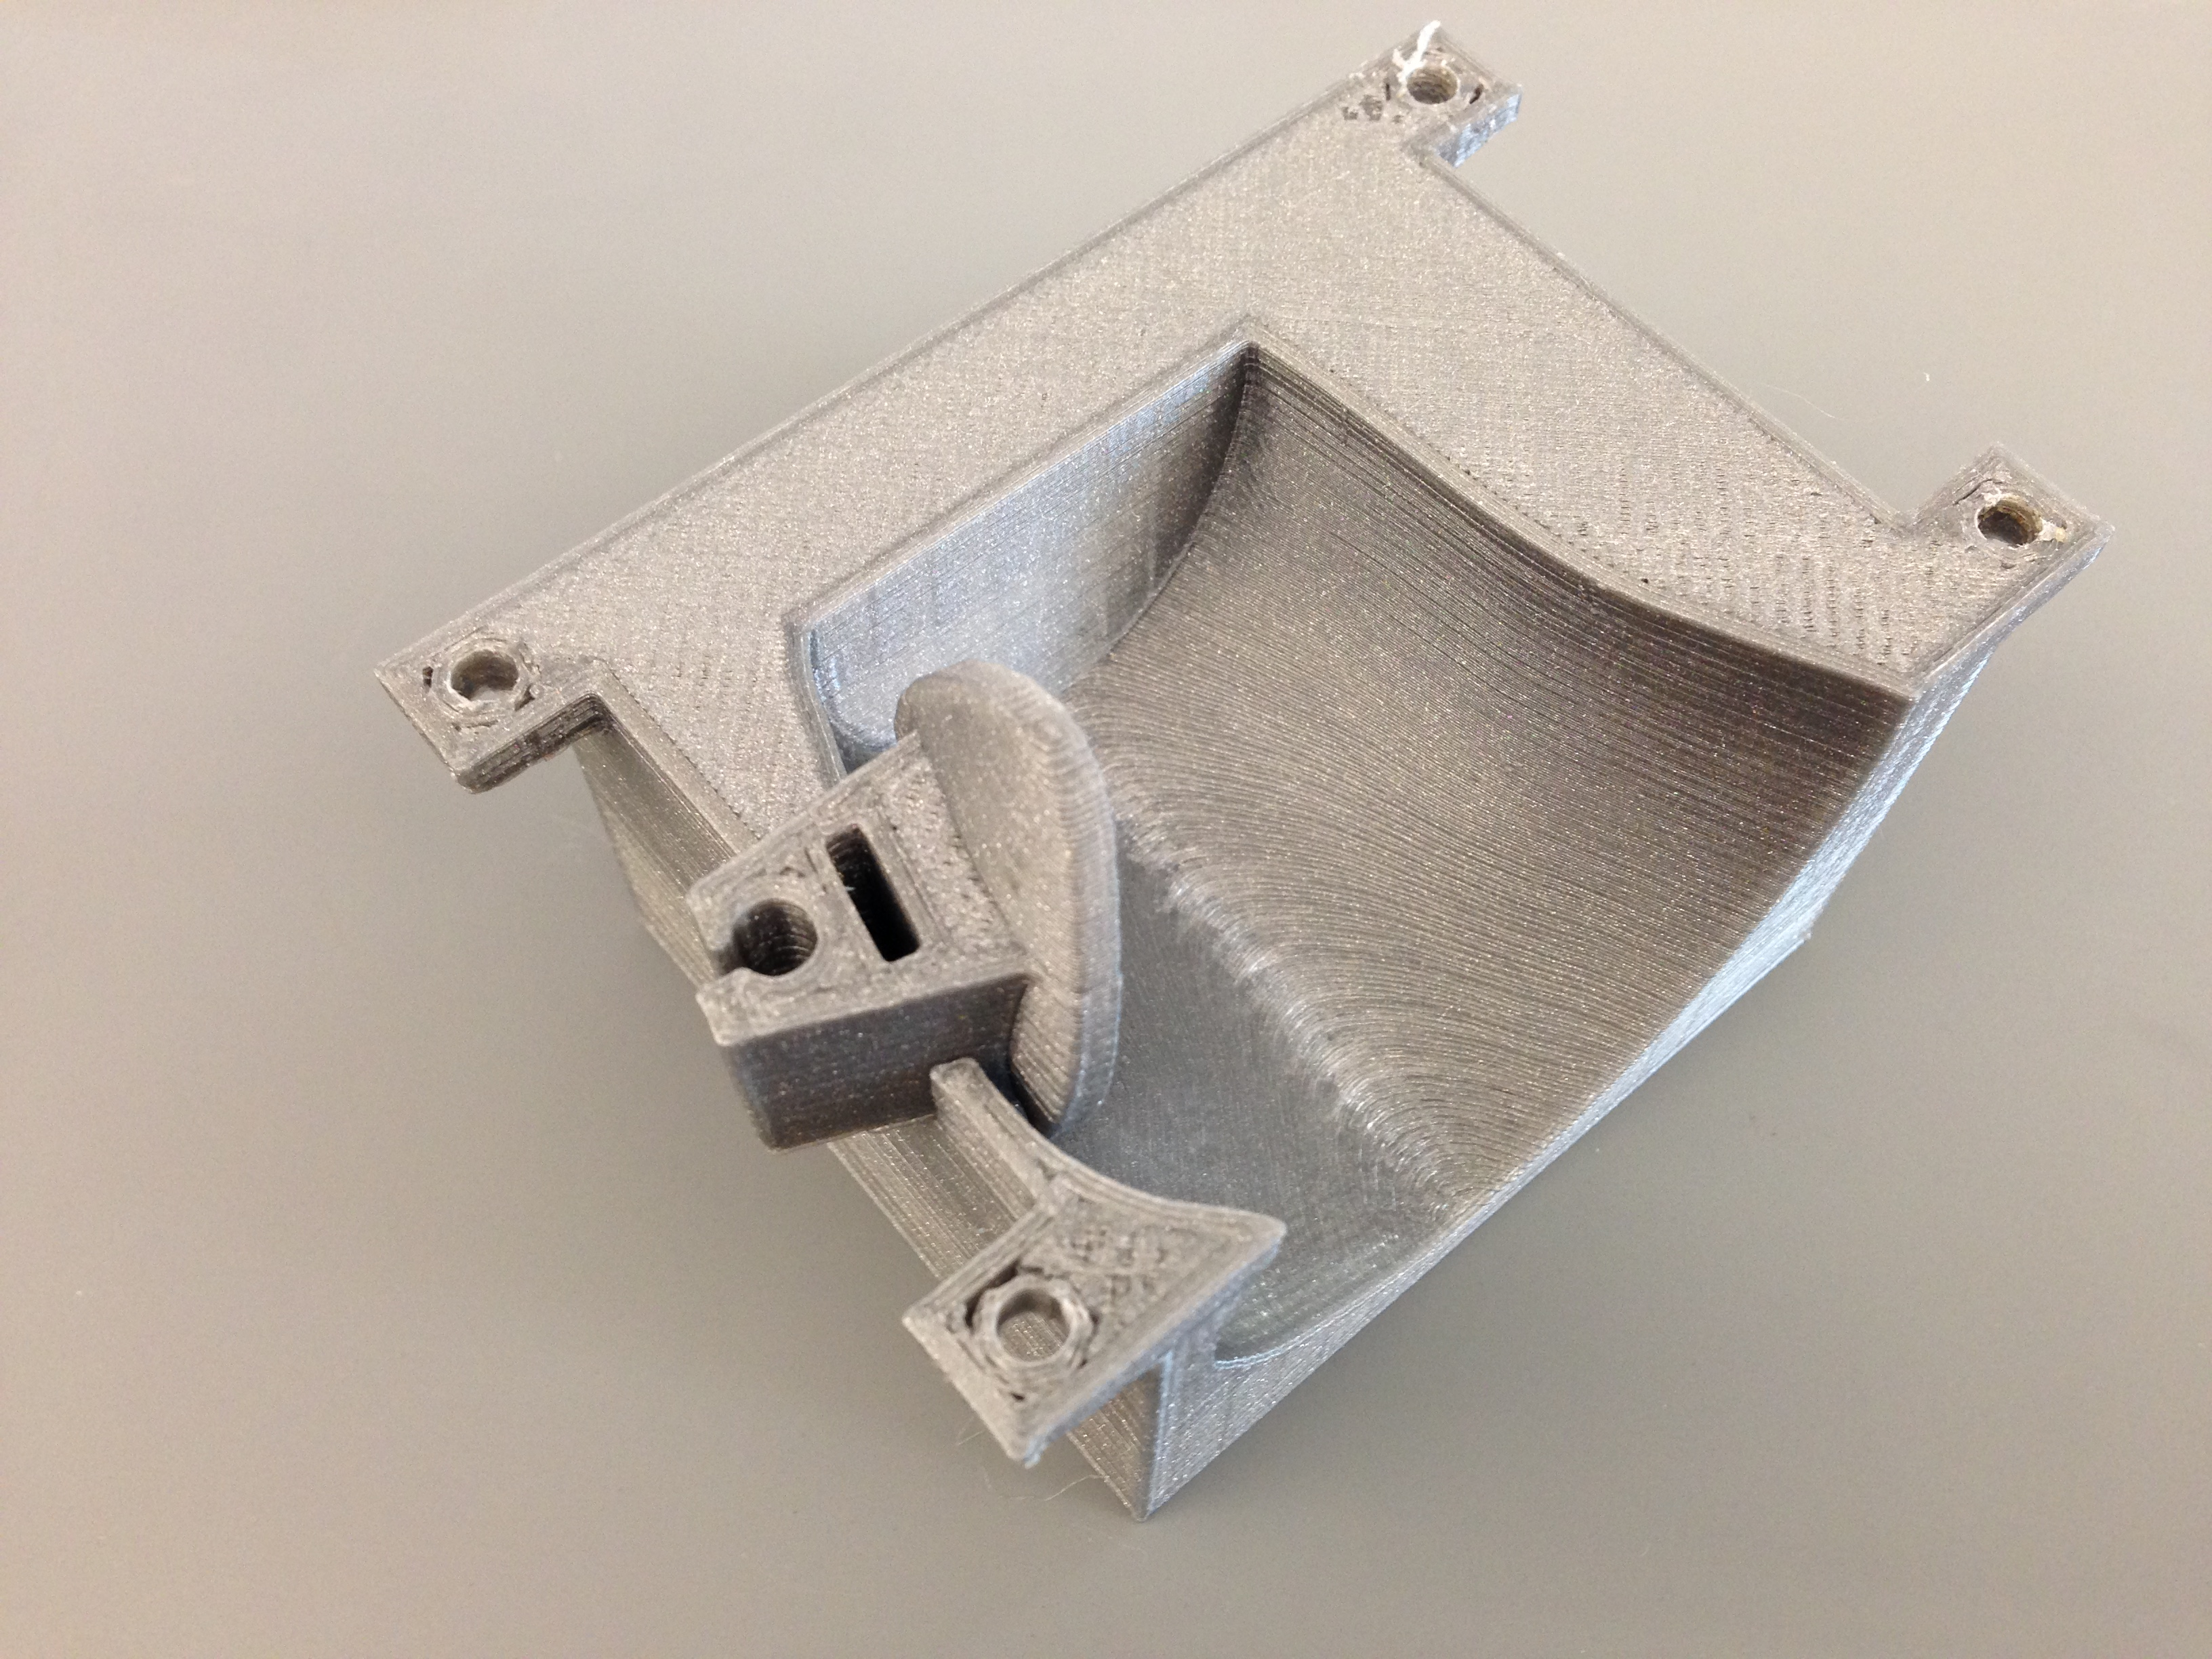
\includegraphics[width=4cm]{images/palm\_mold/moldhalf.jpg}
\item Set the other half of the mold with the flat side up so the two halves align.
\item Fasten the two halves together using the nuts and bolts in the holes at each corner.\\ 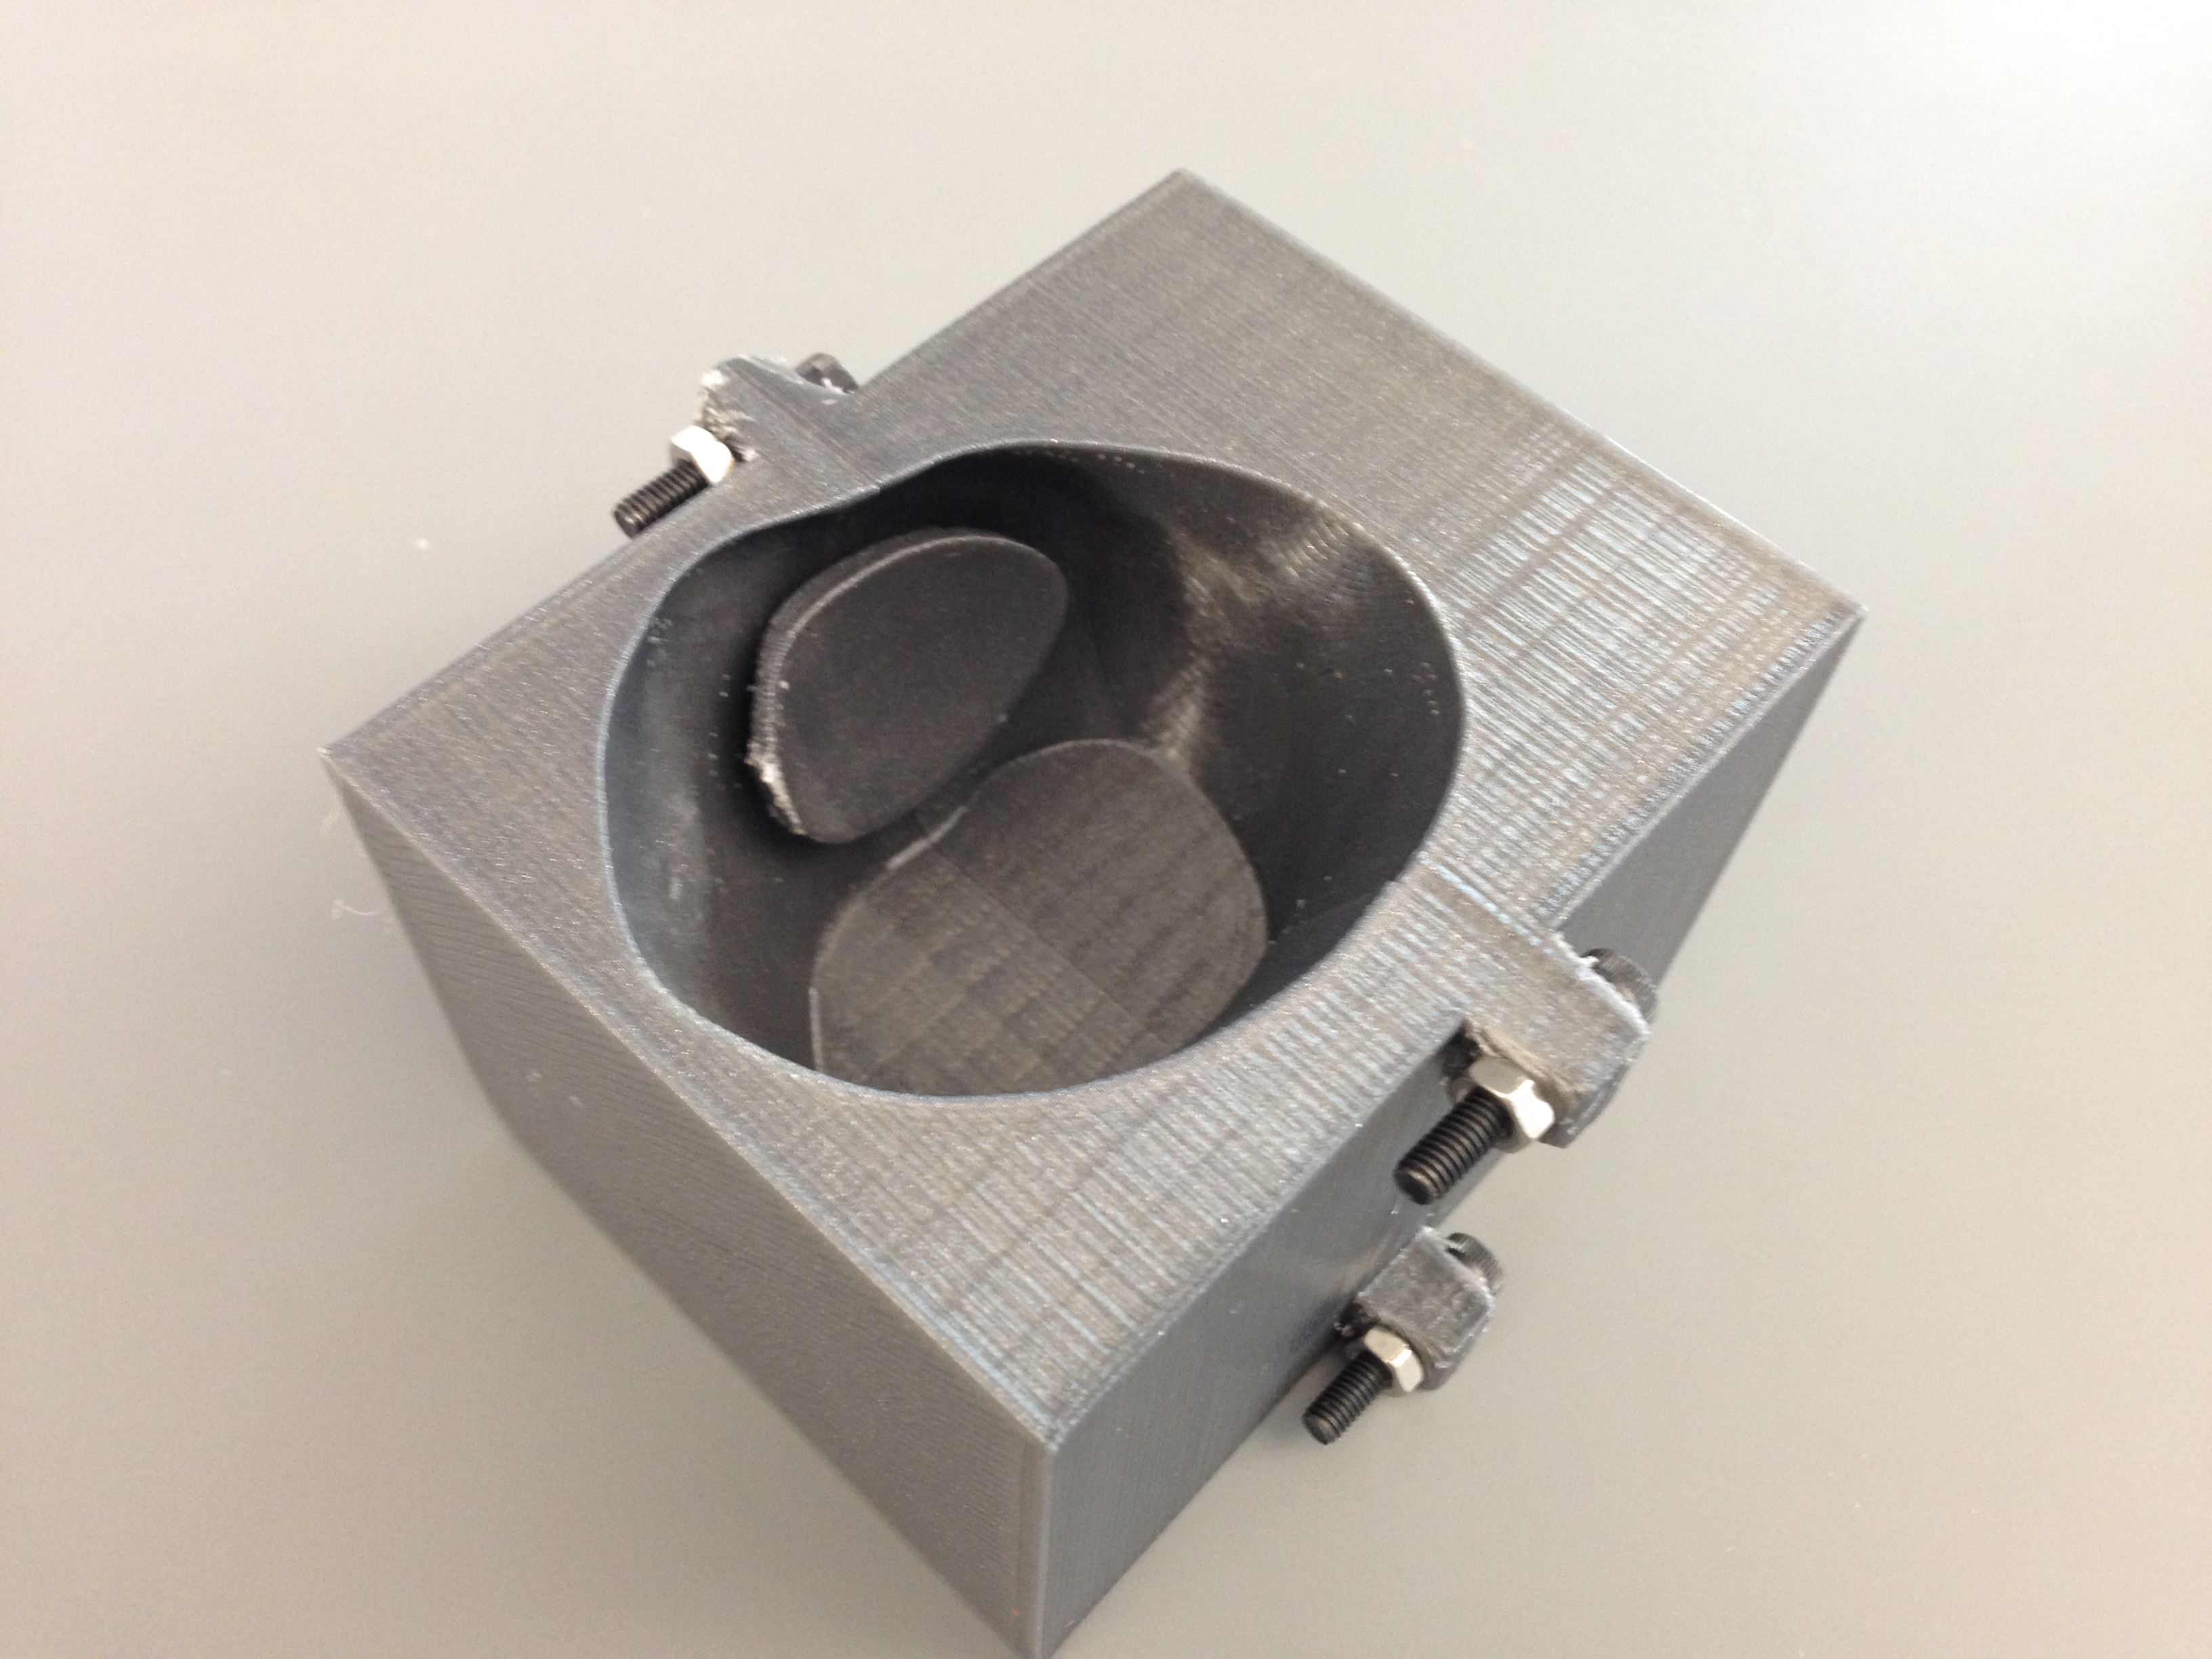
\includegraphics[width=4cm]{images/palm\_mold/assembled.jpg}
\item Optional: use tape to seal the seams on the outside of the mold to prevent leakage.\\ 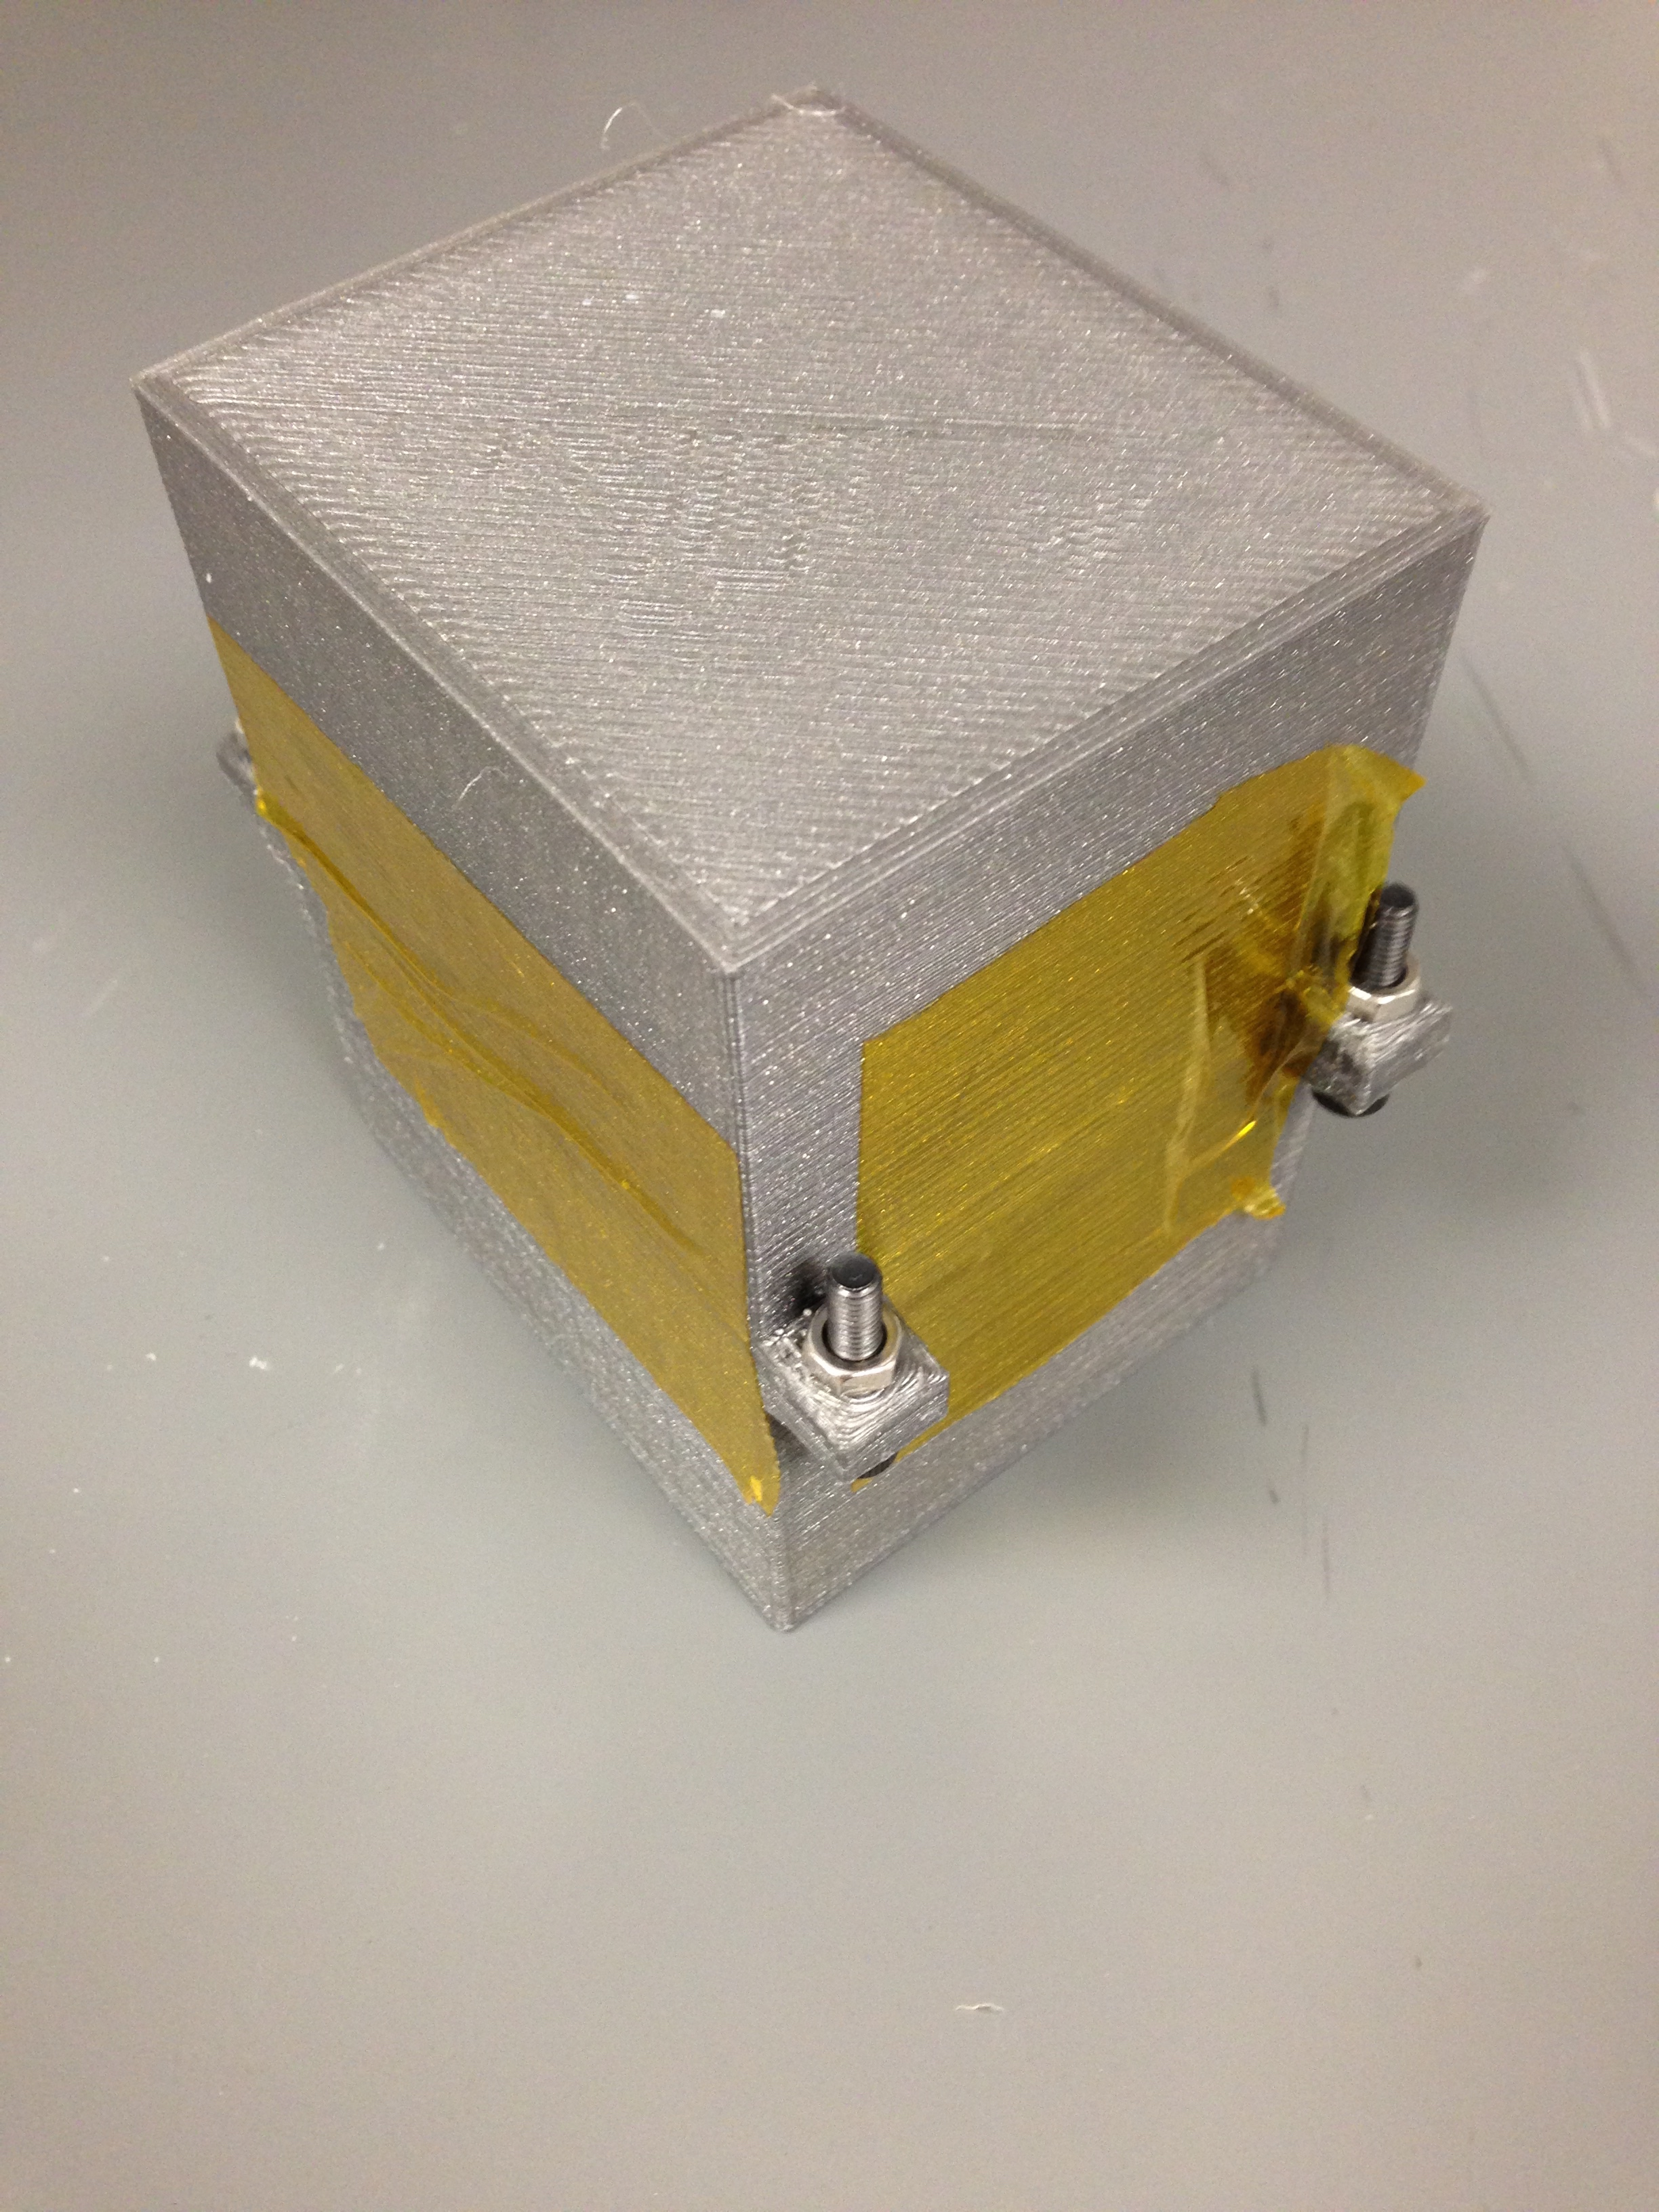
\includegraphics[width=4cm]{images/palm\_mold/taped.jpg}
\end{enumerate}

\subsection{Assemble Silicone sleeve}
Things needed:
\begin{itemize}
\item 100x \hyperlink{thing_g\_dragon\_skin\_30}{grams of Dragon Skin 30 liquid silicone}
\item 1x \hyperlink{thing_mold\_assembly}{Palm Sleeve Mold Assembly}
\item 1x \hyperlink{thing_truncated\_hand}{Truncated Print of Patient's Hand}
\item 2x Piece of Tape
\end{itemize}
Steps:
\begin{enumerate}
\item Mix silicone according to the instructions from the supplier. Wear gloves and follow the supplier's safety guidelines while working with liquid silicone.\\ 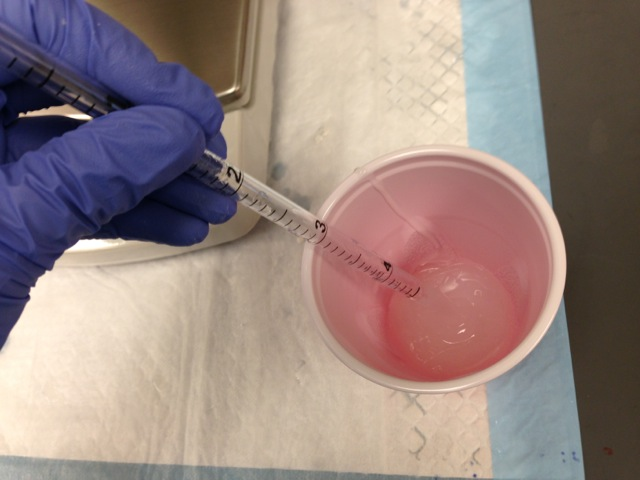
\includegraphics[width=4cm]{images/pad\_casting/Mixing.jpg}
\item Insert the truncated hand in the opening of the mold, narrow side down, so that it sits in the center of the mold and lines up with the overall shape of the mold. Make sure there is a small gap between the truncated hand and the thumb base piece.\\ \includegraphics[width=4cm]{images/palm\_mold/hand\_in\_mold.jpg}
\item Tape the truncated hand in place to prevent it from moving or floating when the silicone is poured. Leave some space around it open to pour the silicone and for air to escape.\\ \includegraphics[width=4cm]{images/palm\_mold/ready\_to\_pour.jpg}
\item Pour the liquid silicone to fill the mold. Make sure it settles to the bottom and completely surrounds the printed hand.\\ 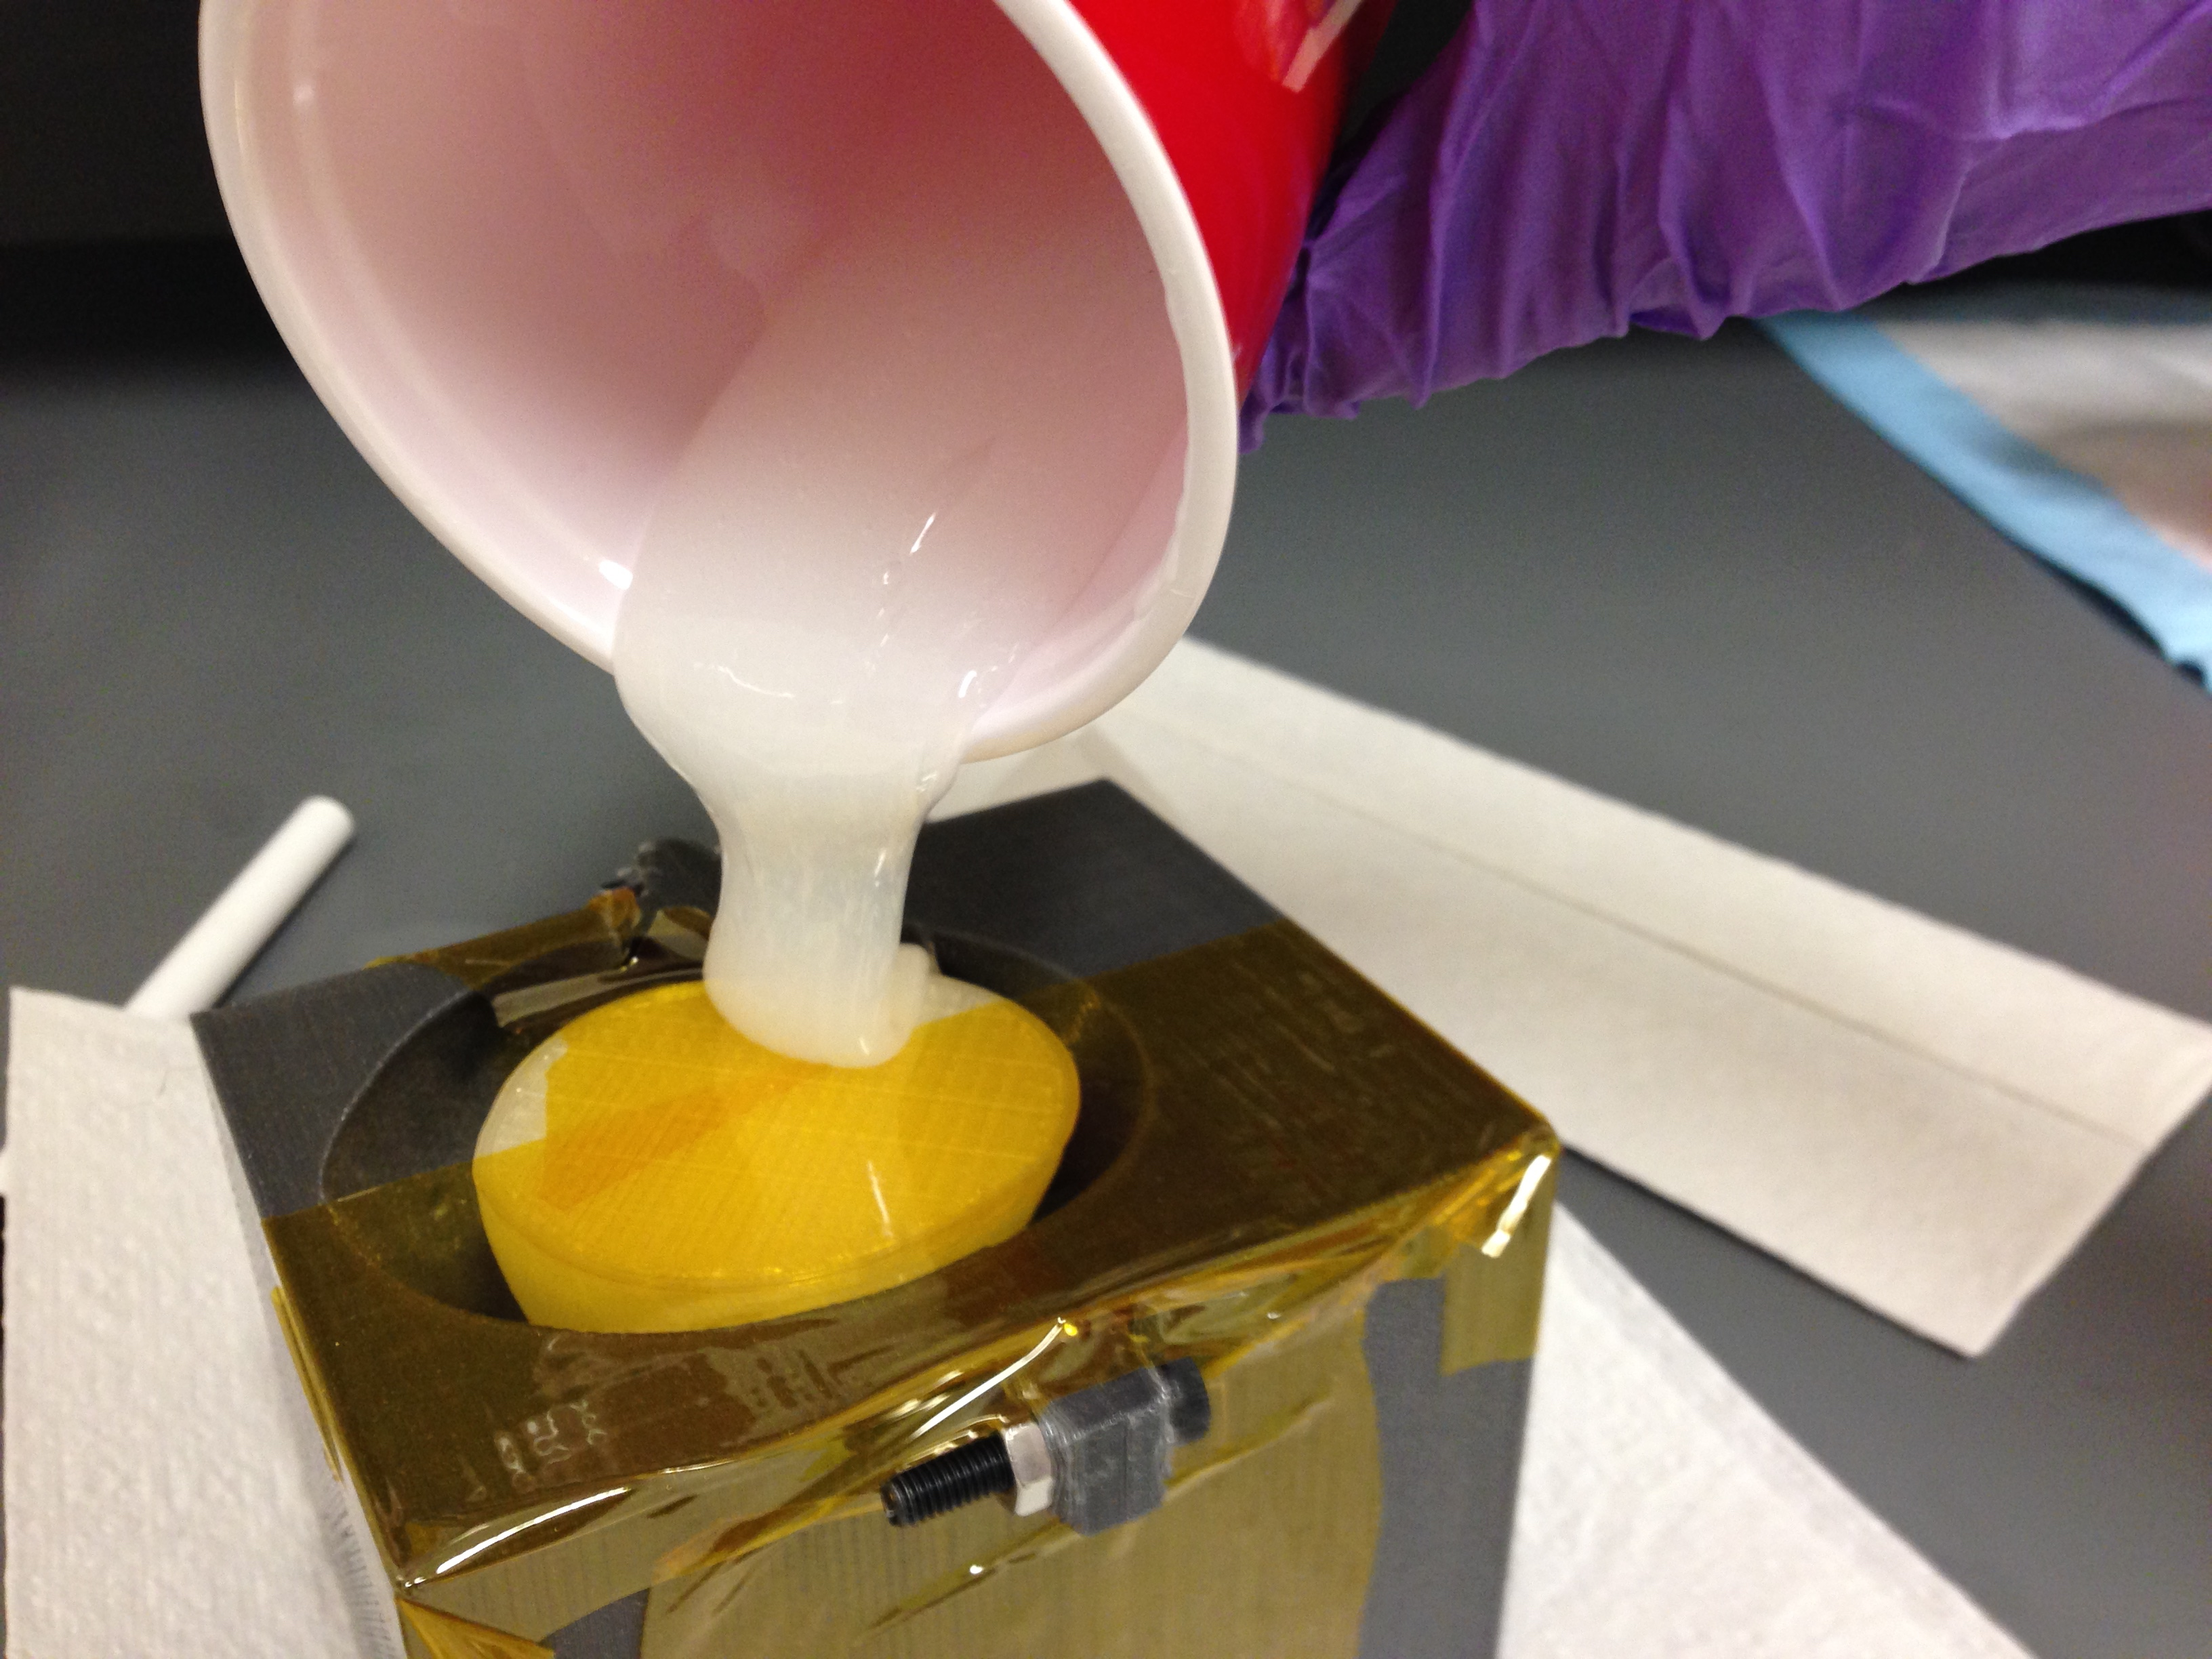
\includegraphics[width=4cm]{images/palm\_mold/pour.jpg}
\item After the silicone cures, unscrew and separate the two halves of the mold, and pull out the truncated hand.
\item If necessary, use a knife to cut off any excess silicone and/or cut the sleeve to better fit the patient's hand.
\end{enumerate}

\subsection{Assemble Thumb with Molded Grip}
Things needed:
\begin{itemize}
\item 1x \hyperlink{thing_rigid\_base}{Rigid base with thumb}
\item 10x \hyperlink{thing_g\_dragon\_skin\_10}{grams of Dragon Skin 10 liquid silicone}
\item 1x \hyperlink{thing_thumb\_mold}{Thumb Mold}
\end{itemize}
Steps:
\begin{enumerate}
\item Print the skeletal thumb and mold.
\item Mix silicone according to the instructions from the supplier. Wear gloves and follow the supplier's safety guidelines while working with liquid silicone.\\ 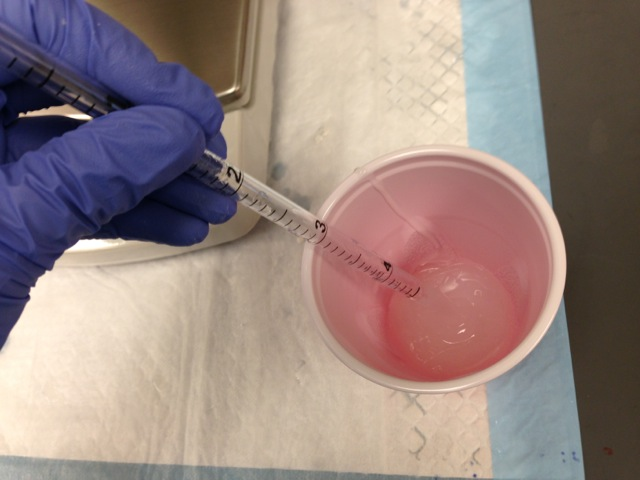
\includegraphics[width=4cm]{images/pad\_casting/Mixing.jpg}
\item Pour the liquid silicone to mostly fill the thumb mold.
\item Insert the printed skeletal thumb into the filled mold as far as it will go.
\item Remove most of the excess silicone. Small amounts of excess can be removed afer molding.
\item After the silicone has cured, carefully pull the thumb to remove it from the mold.
\item If necessary, use a knife to trim off excess silicone so that the edges of the silicone part are flush with those of the hard printed part.
\end{enumerate}

\subsection{Assemble Low Profile Thumb Prosthesis}
Things needed:
\begin{itemize}
\item 1x \hyperlink{thing_silicone\_sleeve}{Silicone sleeve}
\item 1x \hyperlink{thing_molded\_thumb}{Thumb with Molded Grip}
\item 1x \hyperlink{thing_velcro\_strap}{Velcro Strap}
\end{itemize}
Steps:
\begin{enumerate}
\item Insert the thumb into the slot on the base.
\item Insert the velcro strap through the slot on the base.
\item Insert patient's hand into the sleeve.
\item Fasten the velcro strap and tighten as needed to hold the prosthesis in place during use.
\end{enumerate}

\newpage

\end{document}